% This file was created with tikzplotlib v0.10.1.
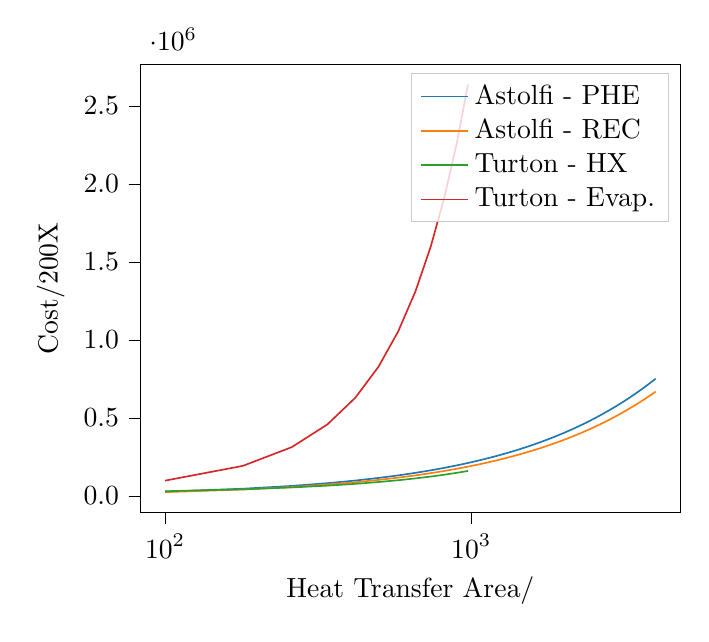
\begin{tikzpicture}

\definecolor{crimson2143940}{RGB}{214,39,40}
\definecolor{darkgray176}{RGB}{176,176,176}
\definecolor{darkorange25512714}{RGB}{255,127,14}
\definecolor{forestgreen4416044}{RGB}{44,160,44}
\definecolor{lightgray204}{RGB}{204,204,204}
\definecolor{steelblue31119180}{RGB}{31,119,180}

\begin{axis}[
legend cell align={left},
legend style={fill opacity=0.8, draw opacity=1, text opacity=1, draw=lightgray204},
log basis x={10},
tick align=outside,
tick pos=left,
unbounded coords=jump,
x grid style={darkgray176},
xlabel={Heat Transfer Area/\unit{\square\m}},
xmin=83.1566529016914, xmax=4810.19841518734,
xmode=log,
xtick style={color=black},
xtick={1,10,100,1000,10000,100000},
xticklabels={
  \(\displaystyle {10^{0}}\),
  \(\displaystyle {10^{1}}\),
  \(\displaystyle {10^{2}}\),
  \(\displaystyle {10^{3}}\),
  \(\displaystyle {10^{4}}\),
  \(\displaystyle {10^{5}}\)
},
y grid style={darkgray176},
ylabel={Cost/\unit{\USD}200X},
ymin=-106486.932070928, ymax=2768057.01361335,
ytick style={color=black},
ytick={-500000,0,500000,1000000,1500000,2000000,2500000,3000000},
yticklabels={\ensuremath{-}0.5,0.0,0.5,1.0,1.5,2.0,2.5,3.0}
]
\addplot [semithick, steelblue31119180]
table {%
100 27179.2373879136
179.591836734694 46035.747544522
259.183673469388 64044.839805698
338.775510204082 81500.0873243671
418.367346938775 98546.0610170705
497.959183673469 115268.764582061
577.551020408163 131725.115124216
657.142857142857 147955.488208465
736.734693877551 163989.966272872
816.326530612245 179851.799308529
895.918367346939 195559.475166005
975.510204081633 211128.033107788
1055.10204081633 226569.936854543
1134.69387755102 241895.677140371
1214.28571428571 257114.200773128
1293.87755102041 272233.224300465
1373.4693877551 287259.46853116
1453.0612244898 302198.837324641
1532.65306122449 317056.556227955
1612.24489795918 331837.281599019
1691.83673469388 346545.187648732
1771.42857142857 361184.036700298
1851.02040816327 375757.236511373
1930.61224489796 390267.887495709
2010.20408163265 404718.8219675
2089.79591836735 419112.637018802
2169.38775510204 433451.72226632
2248.97959183673 447738.283427151
2328.57142857143 461974.36247603
2408.16326530612 476161.854979672
2487.75510204082 490302.525083832
2567.34693877551 504398.018535862
2646.9387755102 518449.874053213
2726.5306122449 532459.533291387
2806.12244897959 546428.349619742
2885.71428571429 560357.595877483
2965.30612244898 574248.471253226
3044.89795918367 588102.107408024
3124.48979591837 601919.573942654
3204.08163265306 615701.883294302
3283.67346938775 629449.995134891
3363.26530612245 643164.820332627
3442.85714285714 656847.224529433
3522.44897959184 670498.031379544
3602.04081632653 684118.025488281
3681.63265306122 697707.955084771
3761.22448979592 711268.534457926
3840.81632653061 724800.446181222
3920.40816326531 738304.343148582
4000 751780.850440909
};
\addlegendentry{Astolfi - PHE}
\addplot [semithick, darkorange25512714]
table {%
100 24174.1563692661
179.591836734694 40945.7904883019
259.183673469388 56963.7017408011
338.775510204082 72489.0042707461
418.367346938775 87650.2844653498
497.959183673469 102524.036996638
577.551020408163 117160.8859117
657.142857142857 131596.742638301
736.734693877551 145858.363540177
816.326530612245 159966.42796577
895.918367346939 173937.379650574
975.510204081633 187784.595036243
1055.10204081633 201519.159788203
1134.69387755102 215150.404729208
1214.28571428571 228686.287460459
1293.87755102041 242133.671347065
1373.4693877551 255498.534109444
1453.0612244898 268786.126844933
1532.65306122449 282001.097336306
1612.24489795918 295147.587109789
1691.83673469388 308229.308853327
1771.42857142857 321249.608907662
1851.02040816327 334211.518250642
1930.61224489796 347117.794497789
2010.20408163265 359970.956807576
2089.79591836735 372773.315123752
2169.38775510204 385526.994854291
2248.97959183673 398233.957840478
2328.57142857143 410896.020285463
2408.16326530612 423514.868172025
2487.75510204082 436092.070592582
2567.34693877551 448629.091331908
2646.9387755102 461127.29897867
2726.5306122449 473587.975791271
2806.12244897959 486012.325503356
2885.71428571429 498401.480222258
2965.30612244898 510756.506547924
3044.89795918367 523078.411018943
3124.48979591837 535368.144975341
3204.08163265306 547626.608913866
3283.67346938775 559854.656400009
3363.26530612245 572053.097591543
3442.85714285714 584222.702420418
3522.44897959184 596364.203473276
3602.04081632653 608478.298605302
3681.63265306122 620565.653317431
3761.22448979592 632626.902922994
3840.81632653061 644662.654526515
3920.40816326531 656673.488834493
4000 668659.961815561
};
\addlegendentry{Astolfi - REC}
\addplot [semithick, forestgreen4416044]
table {%
100 30019.2612224169
179.591836734694 42393.6659108463
259.183673469388 54228.5599169651
338.775510204082 65858.6456854471
418.367346938775 77422.7258728511
497.959183673469 88991.5160959162
577.551020408163 100605.471546057
657.142857142857 112289.502330883
736.734693877551 124059.723857524
816.326530612245 135926.920193759
895.918367346939 147898.471875287
975.510204081633 159979.497802811
1055.10204081633 nan
1134.69387755102 nan
1214.28571428571 nan
1293.87755102041 nan
1373.4693877551 nan
1453.0612244898 nan
1532.65306122449 nan
1612.24489795918 nan
1691.83673469388 nan
1771.42857142857 nan
1851.02040816327 nan
1930.61224489796 nan
2010.20408163265 nan
2089.79591836735 nan
2169.38775510204 nan
2248.97959183673 nan
2328.57142857143 nan
2408.16326530612 nan
2487.75510204082 nan
2567.34693877551 nan
2646.9387755102 nan
2726.5306122449 nan
2806.12244897959 nan
2885.71428571429 nan
2965.30612244898 nan
3044.89795918367 nan
3124.48979591837 nan
3204.08163265306 nan
3283.67346938775 nan
3363.26530612245 nan
3442.85714285714 nan
3522.44897959184 nan
3602.04081632653 nan
3681.63265306122 nan
3761.22448979592 nan
3840.81632653061 nan
3920.40816326531 nan
4000 nan
};
\addlegendentry{Turton - HX}
\addplot [semithick, crimson2143940]
table {%
100 97994.1161095594
179.591836734694 192693.934725923
259.183673469388 312554.119493926
338.775510204082 458084.180645408
418.367346938775 629946.250421208
497.959183673469 828887.630404897
577.551020408163 1055704.97998642
657.142857142857 1311224.87153447
736.734693877551 1596292.6722481
816.326530612245 1911765.88609109
895.918367346939 2258510.01696109
975.510204081633 2637395.92517315
1055.10204081633 nan
1134.69387755102 nan
1214.28571428571 nan
1293.87755102041 nan
1373.4693877551 nan
1453.0612244898 nan
1532.65306122449 nan
1612.24489795918 nan
1691.83673469388 nan
1771.42857142857 nan
1851.02040816327 nan
1930.61224489796 nan
2010.20408163265 nan
2089.79591836735 nan
2169.38775510204 nan
2248.97959183673 nan
2328.57142857143 nan
2408.16326530612 nan
2487.75510204082 nan
2567.34693877551 nan
2646.9387755102 nan
2726.5306122449 nan
2806.12244897959 nan
2885.71428571429 nan
2965.30612244898 nan
3044.89795918367 nan
3124.48979591837 nan
3204.08163265306 nan
3283.67346938775 nan
3363.26530612245 nan
3442.85714285714 nan
3522.44897959184 nan
3602.04081632653 nan
3681.63265306122 nan
3761.22448979592 nan
3840.81632653061 nan
3920.40816326531 nan
4000 nan
};
\addlegendentry{Turton - Evap.}
\end{axis}

\end{tikzpicture}
